\documentclass[14pt]{extreport}

\usepackage{sty/gost}
\usepackage{listings}
\usepackage{longtable,rotating}
\usepackage{threeparttable}
\usepackage{amsmath}

\begin{document}

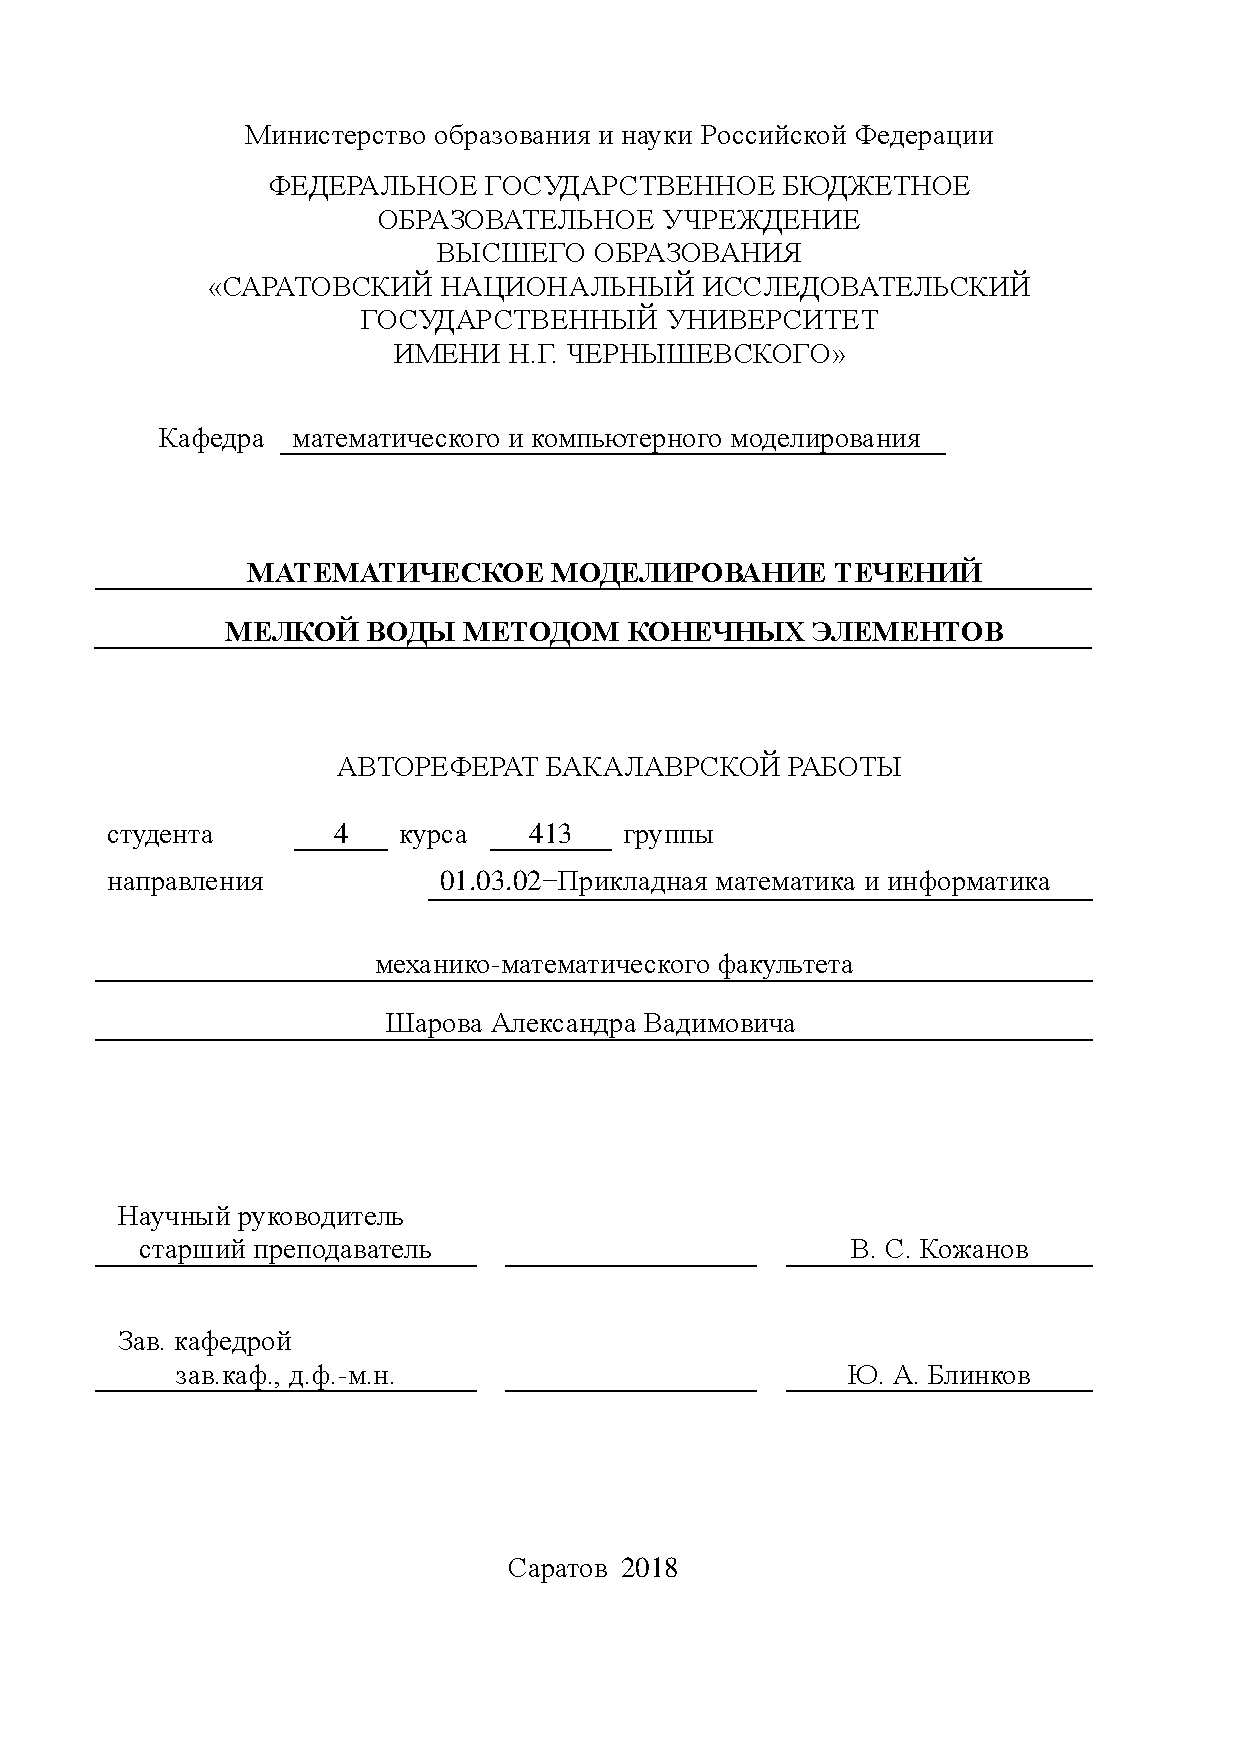
\includepdf[pages={1}]{titul/report.pdf}
%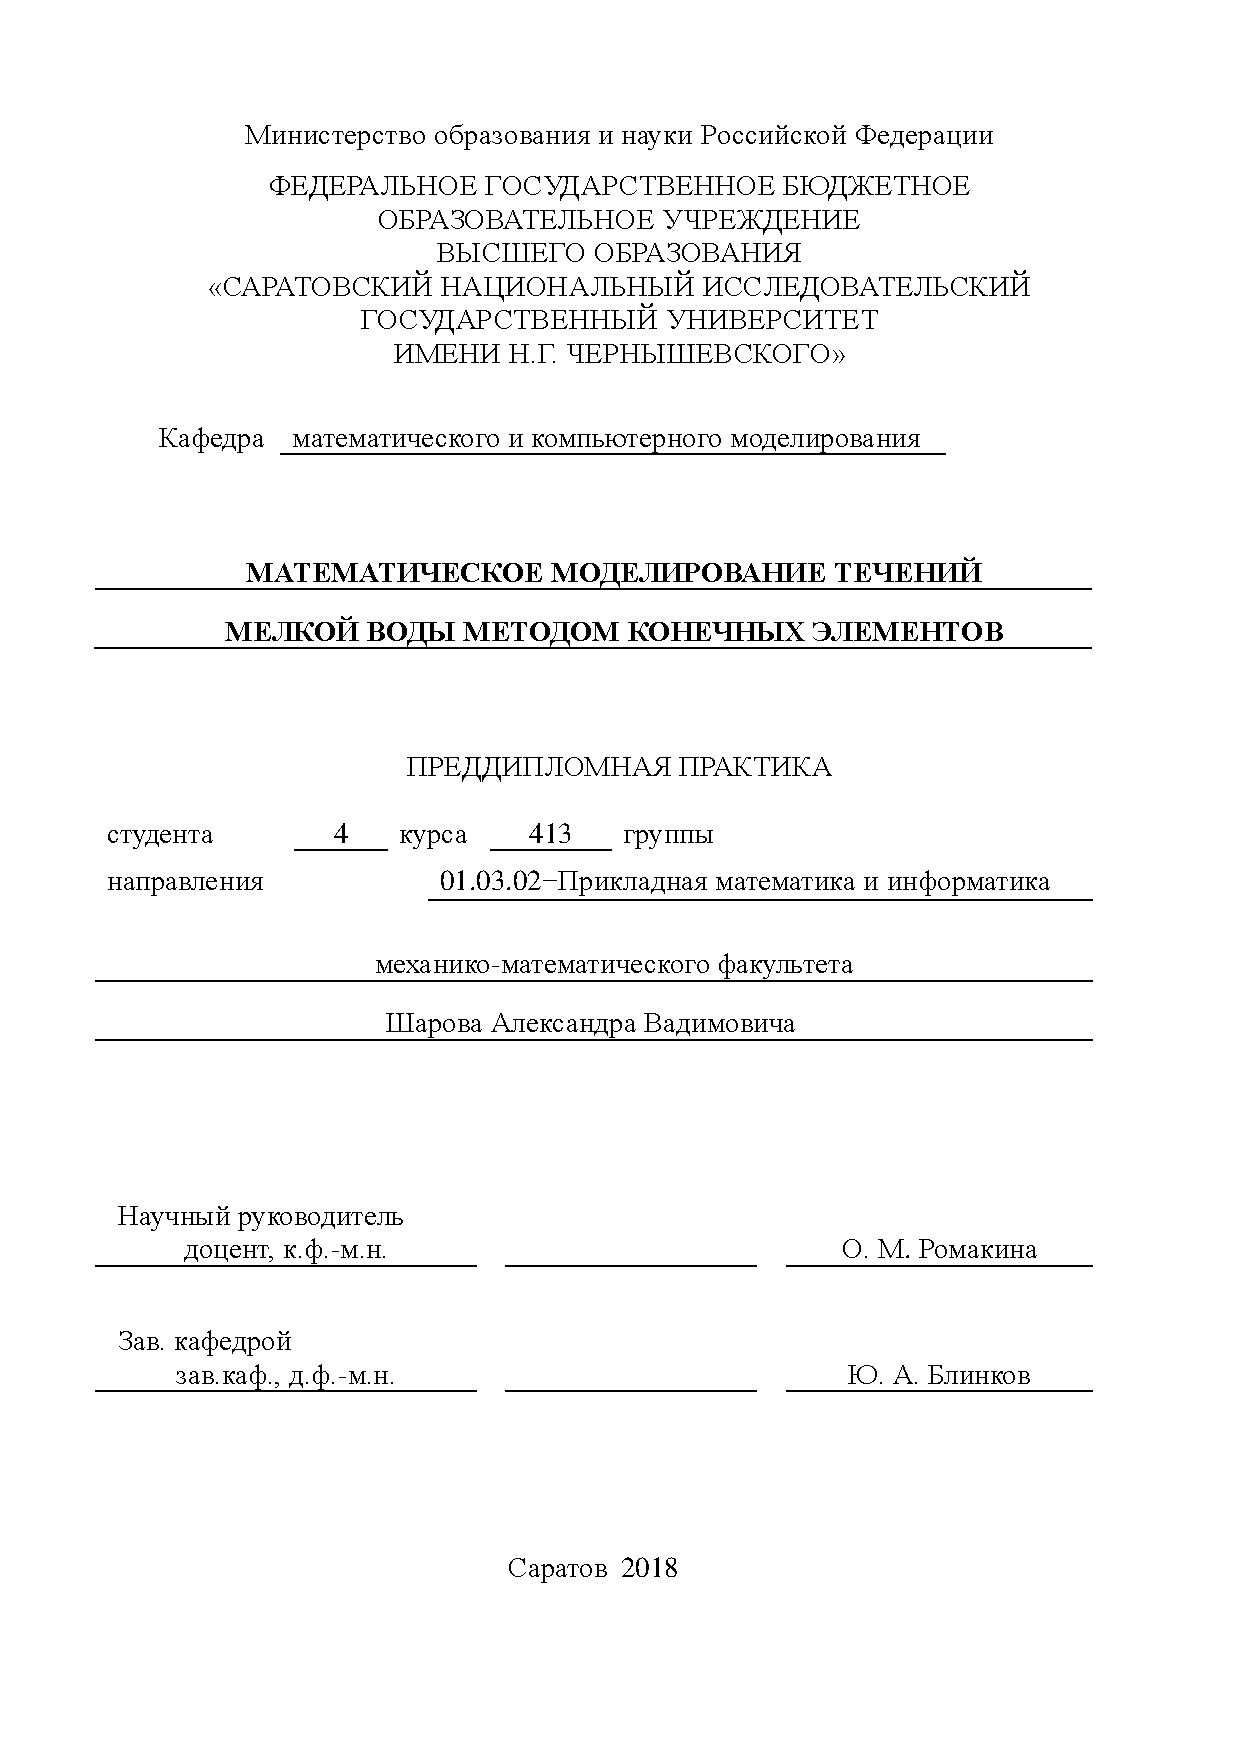
\includepdf[pages={1}]{titul/practice.pdf}

\textbf{Введение}. Для корректного построения математических моделей и численных методов расчета течения жидкости важно знать, каким именно образом описываются основные процессы, происходящие в водоеме. Для этого строятся модели, которые учитывают основные характеристики течения в природной среде.

На данный момент во многих случаях не оправдывается применение более сложных математических моделей для исследования течений в прибрежных водах и озерах, чем модели, полученные путем применения осредненных по вертикали характеристик и основанные на численном решении двумерных уравнений - уравнений мелкой воды.

Уравнения мелкой воды - широко известное приближение, на основе которого проводится численное моделирование течений в реках и водоемах, в прибрежных зонах морей и океанов. Трехмерные решения данных уравнений являются нецелесообразными, так как они требуют намного большего количества исходной информации и машинного времени даже с учетом современных вычислительных мощностей.

При выводе данных уравнений предполагается, что среда представляет собой достаточно тонкий слой, глубина которого много меньше его продольного размера, поэтому вертикальной составляющей скорости можно пренебречь и полагать, что продольные скорости постоянны по толщине слоя.  Исходя из этого данное приближение успешно применяется для описания течений, где влияние на поток свободной поверхности и рельефа дна значительно.

Актуальность данной работы обусловлена тем, что сейчас есть потребность в более точном и быстром решении уже решенных физических задач. Этой потребности отвечает появление новых быстродействующих систем и методов решения. Так, в данной бакалаврской работе была разработана параллельная реализация МКЭ для уравнений МВ, которая позволит более эффективно исследовать различные течения, которые могут быть описаны с помощью уравнений МВ.

Целью представленной выпускной квалификационной работы является построение и численная реализация математической модели на основе двумерных уравнений мелкой воды с помощью метода конечных элементов, который уже давно зарекомендовал себя в таких областях, как механика деформируемого тела, электродинамика и, конечно же, гидродинамика. Данный метод является оптимальным для решения поставленной задачи, так как именно он дает возможность применять достаточно гибкую разбивку рассматриваемой области и при его использовании достаточно удовлетворить лишь главным граничным условиям. Для этой задачи требуется составить и решить систему дифференциальных уравнений с использованием метода конечных элементов. Предполагается, что глубина водоема постоянна, а сам водоем является однородным, то есть не рассматривается случай ГЖС. Необходимо учесть, что озеро подвержено влиянию ветра, а также требуется рассмотреть данную задачу с различными начальными параметрами и проанализировать полученные результаты. Похожая задача для уже решалась ранее, но рассматривался либо только стационарный случай, либо использовались другие методы.

Практическая значимость данной работе представлены основные определения и понятия для уравнений мелкой воды, которые позволяют составить и решить поставленную задачу, состоящую из двух частей: аналитической и численной. Аналитически описаны течения жидкости при пренебрежении температурными эффектами, для которых широко используются классические уравнения Сен-Венана. С помощью МКЭ построена и рассчитана математическая модель МВ. В качестве реализации модели написана программа на языке Python, которая выдает результаты решения системы уравнений мелкой воды, а также строит графики, наглядным образом отображающие полученные результаты.


\textbf{Содержание бакалаврской работы}

\textbf{Вывод уравнений мелкой воды}. Уравнения мелкой воды выводятся из двух основных уравнений для жидкости, а именно уравнения количества движения и уравнения неразрывности:

\begin{equation}\label{eq:shallow_water:1}
-\frac{\partial p}{\partial x_k} + \frac{\partial \tau_{ik}}{\partial x_i} + \rho b_k = \frac{\partial}{\partial x_i}(\rho v_i v_k) + \frac{\partial}{\partial t}(\rho v_k);
\end{equation}

\begin{equation}\label{eq:shallow_water:2}
\frac{D\rho}{Dt}+\rho \frac{\partial v_i}{\partial x_i} =0
\end{equation}

При математическом моделировании движения мелкой воды сложно применять данные уравнения из-за наличия свободной поверхности, изменения границ во время приливов и отливов и вследствие большого количества переменных.

Данных трудностей можно избежать после ряда упрощений, в результате чего получаются уравнения мелкой воды:

\begin{equation}\label{eq:shallow_water:22}
\begin{aligned}
\dfrac{\partial q_1}{\partial t} + \dfrac{\partial}{\partial x_1} \bigg(\dfrac{q_1^2}{H}\bigg)+\dfrac{\partial }{\partial x_2}\bigg(\dfrac{q_1 q_2}{H}\bigg) = \dfrac{\partial}{\partial x_1} (N_{11}-N_p) + \dfrac{\partial N_{12}}{\partial x_2} + B_1; \\
\dfrac{\partial q_2}{\partial t} + \dfrac{\partial}{\partial x_1} \bigg(\dfrac{q_1 q_2}{H}\bigg)+\dfrac{\partial }{\partial x_2}\bigg(\dfrac{q_2^2}{H}\bigg) = \dfrac{\partial}{\partial x_2} (N_{22}-N_p) + \dfrac{\partial N_{12}}{\partial x_2} + B_2,
\end{aligned}
\end{equation}

\noindentгде

\begin{equation*}
\begin{aligned}
B_1=fq_2+\gamma^2\rho_aW^2\cos(\theta)-\bigg(\dfrac{g}{c^2}\bigg)\dfrac{1}{\rho}\dfrac{q_1\sqrt{(q_1^2+q_2^2)}}{H^2} + p_a \dfrac{\partial H}{\partial x_1} + \rho gH\dfrac{\partial h}{\partial x_1}; \\
B_2=-fq_1+\gamma^2\rho_aW^2\sin(\theta)-\bigg(\dfrac{g}{c^2}\bigg)\dfrac{1}{\rho}\dfrac{q_2\sqrt{(q_1^2+q_2^2)}}{H^2} + p_a \dfrac{\partial H}{\partial x_2} + \rho gH\dfrac{\partial h}{\partial x_2}.
\end{aligned}
\end{equation*}

\textbf{Постановка задачи}.Рассматривается течение мелкой воды в закрытом водоеме при учете влияния на этот водоем ветра. Это явление описывается системой дифференциальных уравнений в частных производных, которая состоит из двух уравнений мелкой воды и уравнения неразрывности:

\begin{eqnarray}\label{eq:task:1}
\begin{cases}
\dfrac{ \partial q_i}{\partial x_i} + \dfrac{\partial(\rho H)}{\partial t} = 0 \\
\dfrac{\partial q_1}{\partial t} + \dfrac{\partial}{\partial x_1} \bigg(\dfrac{q_1^2}{H}\bigg)+\dfrac{\partial }{\partial x_2}\bigg(\dfrac{q_1 q_2}{H}\bigg) = \dfrac{\partial}{\partial x_1} (N_{11}-N_p) + \dfrac{\partial N_{12}}{\partial x_2} + B_1 \\
\dfrac{\partial q_2}{\partial t} + \dfrac{\partial}{\partial x_1} \bigg(\dfrac{q_1 q_2}{H}\bigg)+\dfrac{\partial }{\partial x_2}\bigg(\dfrac{q_2^2}{H}\bigg) = \dfrac{\partial}{\partial x_2} (N_{22}-N_p) + \dfrac{\partial N_{12}}{\partial x_2} + B_2
\end{cases}
\end{eqnarray}

\noindentгде

\begin{equation}\label{eq:task:2}
\begin{aligned}
B_1=fq_2+\gamma^2\rho_aW^2\cos(\theta)-\bigg(\dfrac{g}{c^2}\bigg)\dfrac{1}{\rho}\dfrac{q_1\sqrt{(q_1^2+q_2^2)}}{H^2} + p_a \dfrac{\partial H}{\partial x_1} + \rho gH\dfrac{\partial h}{\partial x_1}; \\
B_2=-fq_1+\gamma^2\rho_aW^2\sin(\theta)-\bigg(\dfrac{g}{c^2}\bigg)\dfrac{1}{\rho}\dfrac{q_2\sqrt{(q_1^2+q_2^2)}}{H^2} + p_a \dfrac{\partial H}{\partial x_2} + \rho gH\dfrac{\partial h}{\partial x_2}.
\end{aligned}
\end{equation}

Для данного двумерного случая системы дифференциальных уравнений требуется найти решение с помощью метода конечных элементов. Реализация должна работать с любой произвольно заданной областью. В качестве примеров таких областей должны быть как искусственно вырытые пруды, так и реальные озера. 

 \textbf{Триангуляция двумерной области}. В геометрии триангуляция дискретного множества точек $P\subset {\mathbb  {R}}^{{n+1}}$ в наиболее общем значении — это разбиение  выпуклой оболочки некоторого набора точек, которое представляет собой планарный граф. Одна из фигур разбиения является выпуклой оболочкой разбиваемого множества, а остальные симплексами -  геометрическими фигурами, которые являются $n-$мерным обобщением треугольника. В любой триангуляции ($T$) формально должны выполняться следующие свойства:

	1. любые два симплекса в T пересекаются в общей грани ребра или вершины или вообще не пересекаются;

	2. множество точек, являющихся вершинами симплексов разбиения, совпадает с множеством $P$;
	
	3. нельзя добавить ни одного нового ребра в граф без нарушения планарности.

Одно и то же множество можно триангулировать разными способами. Триангуляция дает тем лучшую аппроксимацию, чем больше её минимальный угол, при этом формируемые симплексы стремятся к равноугольности. Очень важна максимизация минимального угла в вычислительных задачах, когда точность производимых вычислений очень сильно зависит от размера минимального угла триангуляции. Наилучшей в этом смысле триангуляцией является триангуляция Делоне. Простейшим способом её построения является инкрементальный алгоритм, работающий за $o(n^2)$ операций, но он не поддерживает вырожденные случаи, когда $4$ точки из множества лежат на одной окружности: в этом случае триангуляция Делоне не уникальна, и способов разбиения существует несколько, но минимальные углы этих триангуляций равны. Иногда даже минимальный угол триангуляции Делоне оказывается слишком малым для устойчивой работы использующего её алгоритма, и тогда можно произвести улучшение, используя алгоритм Рапперта [J. Ruppert]. При этом будут добавлены новые вершины триангуляции, а также образованы дополнительные треугольники. Стабильность численного алгоритма (метода конечных элементов, к примеру) может возрасти многократно за счет появления нижней границы для углов. 

\textbf{Метод конечных элементов в двумерной области}. Метод конечных элементов - численный метод решения дифференциальных уравнений в частных производных, возникающими при решении задач прикладной физики.
	В его основе лежат две главные идеи: дискретизация исследуемого объекта и кусочно-элементная аппроксимация исследуемых функций (в физической интерпретации - температуры, давления, перемещения и т.д.).

Идея состоит в том, что область, в которой ищется решение дифференциальных уравнений, разбивается на конечное количество элементов. В каждом из элементов произвольно выбирается вид аппроксимирующей функции. Вне своего элемента аппроксимирующая функция равна нулю. Значения функций в узлах являются решением задачи и заранее неизвестны. Коэффициенты аппроксимирующих функций обычно ищутся из условия равенства значения соседних функций на границах между элементами (в узлах). Затем эти коэффициенты выражаются через значения функций в узлах элементов. Составляется система уравнений. Количество уравнений равно количеству неизвестных значений в узлах, на которых ищется решение исходной системы, и прямо пропорционально количеству элементов. Так как каждый из элементов связан с ограниченным количеством соседних, система уравнений имеет разрежённый вид, что упрощает её решение. 

В рассматриваемой системе \ref{eq:task:1}-\ref{eq:task:2} можно пренебречь членами $-fq_{1}$ и $fq_2$, так как коэффициент Кориолиса очень мал, а также конвективными членами. После отбрасывания неучитываемых членов в \ref{eq:task:1}-\ref{eq:task:2} можно перейти к конечно-элементой формулировке. Для этого необходимо представить функции $q_1(x_1, x_2,t) , q_2(x_1, x_2,t), H(x_1, x_2,t)$ как разложения:

\begin{eqnarray}\label{eq:fem:approx}
q_1(x_1, x_2, t) = \sum\limits_{m=1}^{M} a_m(t)N_m(x, y) \\
q_2(x_1, x_2, t) = \sum\limits_{m=1}^{M} a_{m+k}(t)N_m(x, y) \\
H(x_1, x_2, t) = \sum\limits_{m=1}^{M} a_{2\cdot m+k}(t)N_m(x, y)
\end{eqnarray}

Важно заметить, что в данных разложениях применяются одни и те же весовые функции $N_k$.

Следующим шагом необходимо подставить полученные разложения в исходную систему уравнений. После этого каждое из уравнений необходимо умножить на весовую функцию $W_l(x_1, x_2)$ и проинтегрировать во треугольнику. Также каждое из уравнений необходимо разрешить относительно производной, чтобы получить систему обыкновенных дифференциальных уравнений вида:

\begin{eqnarray}
A \cdot \frac{da}{dt} + B \cdot a + \cdots = f
\end{eqnarray}

Важно заметить, что каждое из трех исходных уравнений в частных производных дало по $M$ обыкновенных дифференциальных уравнений, и в конечном итоге задача сводится к решению системы из $3\cdot M$ дифференциальных уравнений.

В данной бакалаврской работе конечная система уравнений не была получена аналитически, так как для упрощения решения и минимизации ошибок был использован программный пакет sympy. С помощью его и системы Jupiter Notebook три формулы для $q_1$, $q_2$ и $H$ соответсвенно  были выведены, а далее запрограммированы с помощью функции solve ivp из пакета scipy и приведены в приложении В.

\textbf{Построение графиков}. Для того чтобы визуализировать результаты численных экспериментов, была написана функция, которая строит графики для $q_1$, $q_2$ и $H$ в различные моменты времени. Для лучшей визуализации был написан алгоритм, который комбинирует данные графики в GIF анимацию. Так как количество графиков для некоторых из примеров было достаточно велико, то для создания анимации в случае некоторых экспериментов пришлось писать данные в буфер обмена напрямую, так как в противном случае происходило переполнение и программа переставала работать.

Все графики строятся по изначальным точкам разбиения области. Для того чтобы получить более детальную картинку, была произведена кубическая интерполяция.

Для получения дополнительной информации об эксперименте была написана функция для визуализации графика функции тока:

$$\Psi = \int q_1(x_1, x_2) dx_2$$

Визуализация данной функции дает лучшее понимание о том, каким именно образом распространяются волны в водоеме. Для данных графиков тоже была произведена кубическая интерполяция.

\textbf{Изменение формы водоема}. В качестве сетки для рассматриваемой задачи сначала был выбран квадратный пруд. После этого сетка была усложнена добавлением в пруд двух островов. После тестирования алгоритма на этой сетке с помощью сервиса openstreetmap была составлена сетка для реального озера Эльтон, а в последствии и для озера Верхнее.

\textbf{Разработка базы данных для хранения информации о проведённых экспериментах}. Данные, полученные в результате численных экспериментов, являются разрозненными, так как они представляют из себя не только GIF анимацию, но и некоторую метаинформацию, которая представлена в виде JSON файлов. Из-за этого, помимо общепринятых требований к БД, следует основываясь на приведенной выше специфике данных, которые были получены в результате решения поставленной задачи, ввести следующие требования, которым должны удовлетворять БД и СУБД, управляющая ей:

\begin{enumerate}

\item Запись об эксперименте должна позволять хранить любую метаинформацию, которая может различаться в зависимости от проведенного эксперимента

\item БД должна позволять добавлять поля к уже существующим данным. Это, к примеру, нужно для добавления в запись данных, которые получены в результате постобработки эксперимента человеком

\item БД должна легко масштабироваться, так как данных может быть много

\item Должно быть отсутствие необходимости сопоставления объекта в базе и программе для упрощения разработки

\item Хранение графической информации должно быть реализовано максимально просто и эффективно

\end{enumerate}

Основной и единственной базой данных является база <<эксперименты>> (<<experiments>>). В ней находится коллекция  <<данные>> (<<data>>). Данная коллекция содержит в себе документы, каждый из которых является проведенным экспериментов. Каждый из документов хранит в себе следующие поля:

\begin{enumerate}
\item дата проведения эксперимента
\item время выполнения эксперимента
\item уникальный идентификатор, указывающий на изображения, полученные в результате экспериментов, которые хранятся в GridFS
\item матрица решения системы ОДУ
\item вектор, хранящий в себе моменты времени, в которых была решена ОДУ
\item тип и файл сетки
\item количество базисных функций
\end{enumerate}

\conclusions
\par В представленной бакалаврской работе были получены уравнения мелкой воды при пренебрежении температурными эффектами, а также написана многопоточная программная реализация МКЭ для решений данных уравнений.

Реализована возможность переносимости разработанного алгоритма, а также возможность его удаленного использования посредством контейнеризации.

В качестве примера были произведены расчеты на различных сетках, в том числе и на реальных озерах(Эльтон и Верхнее). Для данных расчетов были построены графики функций потока жидкости, тока и высоты поверхности. Благодаря этому удалось качественно оценить полученные результаты проведенных экспериментов.



\end{document}